\chapter{Problema}


\section{\fud{} original}

Como ya dijimos incontables veces, \rc{} se acopló sobre el framework de distribución \fud, el cuál fue desarrollado
íntegramente, como trabajo de tesis, por el Lic. Guillermo Biset y el mismo posee vasta documentación en \cite{clus09}.
En la sección \ref{sec:fud} introducimos esta librería y, en distintas secciones del informe, se fueron aportando datos
importantes de como es su funcionamiento en general.\\

Uno de los principios básicos del funcionamiento de \fud{} se basa en el procesamiento aislado de un cliente, es decir,
un cliente conectado recibe su trabajo, mientras lo realiza ignora cualquier tipo de mensaje que pueda llegar a arriba
desde el servidor. Una vez terminado el trabajo envía el resultado correspondiente al servidor. Luego el servidor,
registra a este cliente como libre, implicando su disponibilidad para un nuevo trabajo. Por lo tanto, la comunicación
entre servidor-cliente consta de solo dos interacciones.\\

En las figuras \ref{FuDServerOrig} y \ref{FuDClientOrig} se muestra un diagrama de actividad de la dinámica de los
componentes más importantes de \fud{} original tanto de lado servidor como de cliente respectivamente. Cabe destacar
que en ellos se obviaron aspectos de concurrencia con el fin de no dificultar la visualización el diagrama, se muestra
un solo hilo de ejecución donde un servidor envía un trabajo a un nodo y solamente espera de él su resultado
correspondiente.

    \begin{figure}[ht]
        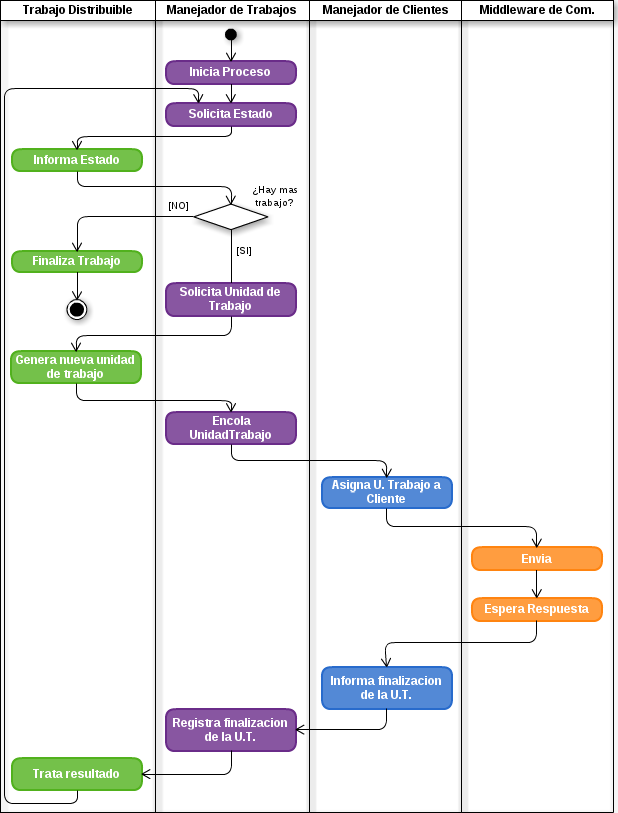
\includegraphics[scale=0.65]{images/ActivityFuDServer-Orig.png}
        \caption{Diagrama de Actividad de \fud{} versión original lado servidor}
            \label{FuDServerOrig}
    \end{figure}

    \begin{figure}[ht]
        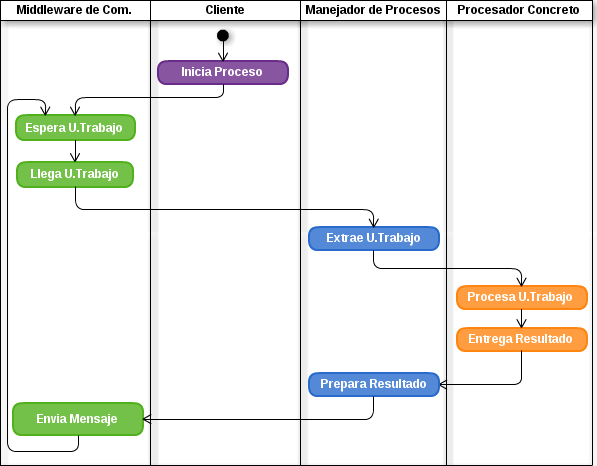
\includegraphics[scale=0.70]{images/ActivityFuDClient-Orig.png}
        \caption{Diagrama de Actividad de \fud{} versión original lado cliente}
            \label{FuDClientOrig}
    \end{figure}



\section{Descripción del Problema}

\rc{} requiere interacción entre servidor y cliente en el transcurso del procesamiento de un trabajo. Ésto se debe a que la generación de
nuevas unidades de trabajo depende exclusivamente de la distribución de trabajo no computado por parte de los clientes, disminuyendo su
carga de trabajo. Un cliente antes de delegar trabajo al servidor necesita también una comunicación previa para conocer si
el servidor tiene disponibilidad de clientes ociosos. Además \rc{} permite el envío de resultados y mensajes en cualquier momento.

Por la naturaleza de \fud{} original era imposible disponer con esta interactividad para poder llevar acabo todas las operaciones antes
descritas, razón que motivó a la refactorización del framework.

